\chapter{Matrices}

\index{matrix}

Una \key{matriz} es un concepto matemático
que corresponde a una matriz bidimensional
en programación. Por ejemplo,
\[
A = 
 \begin{bmatrix}
  6 & 13 & 7 & 4 \\
  7 & 0 & 8 & 2 \\
  9 & 5 & 4 & 18 \\
 \end{bmatrix}
\]
es una matriz de tamaño $3 \times 4$, es decir,
tiene 3 filas y 4 columnas.
La notación $[i,j]$ se refiere a
el elemento en la fila $i$ y la columna $j$
en una matriz.
Por ejemplo, en la matriz anterior,
$A[2,3]=8$ y $A[3,1]=9$.

\index{vector}

Un caso especial de una matriz es un \key{vector}
que es una matriz unidimensional de tamaño $n \times 1$.
Por ejemplo,
\[
V =
\begin{bmatrix}
4 \\
7 \\
5 \\
\end{bmatrix}
\]
es un vector que contiene tres elementos.

\index{transpose}

La \key{transpuesta} $A^T$ de una matriz $A$
se obtiene cuando las filas y columnas de $A$
se intercambian, es decir, $A^T[i,j]=A[j,i]$:
\[
A^T = 
 \begin{bmatrix}
  6 & 7 & 9 \\
  13 & 0 & 5 \\
  7 & 8 & 4 \\
  4 & 2 & 18 \\
 \end{bmatrix}
\]

\index{square matrix}

Una matriz es una \key{matriz cuadrada} si
tiene el mismo número de filas y columnas.
Por ejemplo, la siguiente matriz es una
matriz cuadrada:

\[
S = 
 \begin{bmatrix}
  3 & 12 & 4  \\
  5 & 9 & 15  \\
  0 & 2 & 4 \\
 \end{bmatrix}
\]

\section{Operaciones}

La suma $A+B$ de las matrices $A$ y $B$
se define si las matrices son del mismo tamaño.
El resultado es una matriz donde cada elemento
es la suma de los elementos correspondientes
en $A$ y $B$.

Por ejemplo,
\[
 \begin{bmatrix}
  6 & 1 & 4 \\
  3 & 9 & 2 \\
 \end{bmatrix}
+
 \begin{bmatrix}
  4 & 9 & 3 \\
  8 & 1 & 3 \\
 \end{bmatrix}
=
 \begin{bmatrix}
  6+4 & 1+9 & 4+3 \\
  3+8 & 9+1 & 2+3 \\
 \end{bmatrix}
=
 \begin{bmatrix}
  10 & 10 & 7 \\
  11 & 10 & 5 \\
 \end{bmatrix}.
\]

Multiplicar una matriz $A$ por un valor $x$ significa
que cada elemento de $A$ se multiplica por $x$.
Por ejemplo,
\[
 2 \cdot \begin{bmatrix}
  6 & 1 & 4 \\
  3 & 9 & 2 \\
 \end{bmatrix}
=
 \begin{bmatrix}
  2 \cdot 6 & 2\cdot1 & 2\cdot4 \\
  2\cdot3 & 2\cdot9 & 2\cdot2 \\
 \end{bmatrix}
=
 \begin{bmatrix}
  12 & 2 & 8 \\
  6 & 18 & 4 \\
 \end{bmatrix}.
\]

\subsubsection{Multiplicación de matrices}

\index{matrix multiplication}

El producto $AB$ de las matrices $A$ y $B$
se define si $A$ es de tamaño $a \times n$
y $B$ es de tamaño $n \times b$, es decir,
el ancho de $A$ es igual a la altura de $B$.
El resultado es una matriz de tamaño $a \times b$
cuyos elementos se calculan utilizando la fórmula
\[
AB[i,j] = \sum_{k=1}^n A[i,k] \cdot B[k,j].
\]

La idea es que cada elemento de $AB$
es una suma de productos de elementos de $A$ y $B$
de acuerdo con la siguiente imagen:

\begin{center}
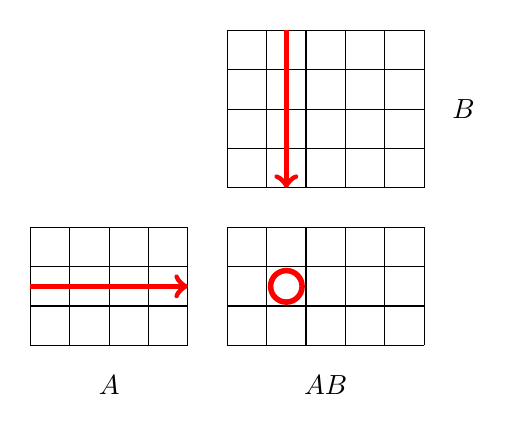
\begin{tikzpicture}[scale=0.5]
\draw (0,0) grid (4,3);
\draw (5,0) grid (10,3);
\draw (5,4) grid (10,8);

\node at (2,-1) {$A$};
\node at (7.5,-1) {$AB$};
\node at (11,6) {$B$};

\draw[thick,->,red,line width=2pt] (0,1.5) -- (4,1.5);
\draw[thick,->,red,line width=2pt] (6.5,8) -- (6.5,4);
\draw[thick,red,line width=2pt] (6.5,1.5) circle (0.4);
\end{tikzpicture}
\end{center}

Por ejemplo,

\[
 \begin{bmatrix}
  1 & 4 \\
  3 & 9 \\
  8 & 6 \\
 \end{bmatrix}
\cdot
 \begin{bmatrix}
  1 & 6 \\
  2 & 9 \\
 \end{bmatrix}
=
 \begin{bmatrix}
  1 \cdot 1 + 4 \cdot 2 & 1 \cdot 6 + 4 \cdot 9 \\
  3 \cdot 1 + 9 \cdot 2 & 3 \cdot 6 + 9 \cdot 9 \\
  8 \cdot 1 + 6 \cdot 2 & 8 \cdot 6 + 6 \cdot 9 \\
 \end{bmatrix}
=
 \begin{bmatrix}
  9 & 42 \\
  21 & 99 \\
  20 & 102 \\
 \end{bmatrix}.
\]

La multiplicación de matrices es asociativa,
por lo que $A(BC)=(AB)C$ se cumple,
pero no es conmutativa,
por lo que $AB = BA$ no suele cumplirse.

\index{identity matrix}

Una \key{matriz identidad} es una matriz cuadrada
donde cada elemento en la diagonal es 1
y todos los demás elementos son 0.
Por ejemplo, la siguiente matriz
es la matriz identidad $3 \times 3$:
\[
 I = \begin{bmatrix}
  1 & 0 & 0 \\
  0 & 1 & 0 \\
  0 & 0 & 1 \\
 \end{bmatrix}
\]

\begin{samepage}
Multiplicar una matriz por una matriz identidad
no la cambia. Por ejemplo,
\[
 \begin{bmatrix}
  1 & 0 & 0 \\
  0 & 1 & 0 \\
  0 & 0 & 1 \\
 \end{bmatrix}
\cdot
 \begin{bmatrix}
  1 & 4 \\
  3 & 9 \\
  8 & 6 \\
 \end{bmatrix}
=
 \begin{bmatrix}
  1 & 4 \\
  3 & 9 \\
  8 & 6 \\
 \end{bmatrix} \hspace{10px} \textrm{y} \hspace{10px}
 \begin{bmatrix}
  1 & 4 \\
  3 & 9 \\
  8 & 6 \\
 \end{bmatrix}
\cdot
 \begin{bmatrix}
  1 & 0 \\
  0 & 1 \\
 \end{bmatrix}
=
 \begin{bmatrix}
  1 & 4 \\
  3 & 9 \\
  8 & 6 \\
 \end{bmatrix}.
\]
\end{samepage}

Usando un algoritmo sencillo,
podemos calcular el producto de
dos matrices $n \times n$
en tiempo $O(n^3)$.
También existen algoritmos más eficientes
para la multiplicación de matrices\footnote{El primer algoritmo de este tipo
fue el algoritmo de Strassen,
publicado en 1969 \cite{str69},
cuya complejidad temporal es $O(n^{2.80735})$;
el mejor algoritmo actual \cite{gal14}
funciona en tiempo $O(n^{2.37286})$},
pero son principalmente de interés teórico
y tales algoritmos no son necesarios
en programación competitiva.


\subsubsection{Potencia de matriz}

\index{matrix power}

La potencia $A^k$ de una matriz $A$ se define
si $A$ es una matriz cuadrada.
La definición se basa en la multiplicación de matrices:
\[ A^k = \underbrace{A \cdot A \cdot A \cdots A}_{\textrm{$k$ times}} \]
Por ejemplo,

\[
 \begin{bmatrix}
  2 & 5 \\
  1 & 4 \\
 \end{bmatrix}^3 =
 \begin{bmatrix}
  2 & 5 \\
  1 & 4 \\
 \end{bmatrix} \cdot
 \begin{bmatrix}
  2 & 5 \\
  1 & 4 \\
 \end{bmatrix} \cdot
 \begin{bmatrix}
  2 & 5 \\
  1 & 4 \\
 \end{bmatrix} =
 \begin{bmatrix}
  48 & 165 \\
  33 & 114 \\
 \end{bmatrix}.
\]
Además, $A^0$ es una matriz identidad. Por ejemplo,
\[
 \begin{bmatrix}
  2 & 5 \\
  1 & 4 \\
 \end{bmatrix}^0 =
 \begin{bmatrix}
  1 & 0 \\
  0 & 1 \\
 \end{bmatrix}.
\]

La matriz $A^k$ puede calcularse eficientemente
en tiempo $O(n^3 \log k)$ usando el
algoritmo en el Capítulo 21.2. Por ejemplo,
\[
 \begin{bmatrix}
  2 & 5 \\
  1 & 4 \\
 \end{bmatrix}^8 =
 \begin{bmatrix}
  2 & 5 \\
  1 & 4 \\
 \end{bmatrix}^4 \cdot
 \begin{bmatrix}
  2 & 5 \\
  1 & 4 \\
 \end{bmatrix}^4.
\]

\subsubsection{Determinante}

\index{determinant}

El \key{determinante} $\det(A)$ de una matriz $A$
se define si $A$ es una matriz cuadrada.
Si $A$ es de tamaño $1 \times 1$,
entonces $\det(A)=A[1,1]$.
El determinante de una matriz más grande es
calculado recursivamente usando la fórmula \index{cofactor}
\[\det(A)=\sum_{j=1}^n A[1,j] C[1,j],\]
donde $C[i,j]$ es el \key{cofactor} de $A$
en $[i,j]$.
El cofactor se calcula usando la fórmula
\[C[i,j] = (-1)^{i+j} \det(M[i,j]),\]
donde $M[i,j]$ se obtiene eliminando
la fila $i$ y la columna $j$ de $A$.
Debido al coeficiente $(-1)^{i+j}$ en el cofactor,
cada determinante alternativo es positivo
y negativo.
Por ejemplo,
\[
\det(
 \begin{bmatrix}
  3 & 4 \\
  1 & 6 \\
 \end{bmatrix}
) = 3 \cdot 6 - 4 \cdot 1 = 14 
\]
y
\[
\det(
 \begin{bmatrix}
  2 & 4 & 3 \\
  5 & 1 & 6 \\
  7 & 2 & 4 \\
 \end{bmatrix}
) = 
2 \cdot
\det(
 \begin{bmatrix}
  1 & 6 \\
  2 & 4 \\
 \end{bmatrix}
)
-4 \cdot
\det(
 \begin{bmatrix}
  5 & 6 \\
  7 & 4 \\
 \end{bmatrix}
)
+3 \cdot
\det(
 \begin{bmatrix}
  5 & 1 \\
  7 & 2 \\
 \end{bmatrix}
) = 81.
\]

\index{inverse matrix}

El determinante de $A$ nos dice
si existe una \key{matriz inversa}
$A^{-1}$ tal que $A \cdot A^{-1} = I$,
donde $I$ es una matriz identidad.
Resulta que $A^{-1}$ existe
exactamente cuando $\det(A) \neq 0$,
y se puede calcular usando la fórmula

\[A^{-1}[i,j] = \frac{C[j,i]}{det(A)}.\]

Por ejemplo,

\[
\underbrace{
 \begin{bmatrix}
  2 & 4 & 3\\
  5 & 1 & 6\\
  7 & 2 & 4\\
 \end{bmatrix}
}_{A}
\cdot
\underbrace{
 \frac{1}{81}
 \begin{bmatrix}
   -8 & -10 & 21 \\
   22 & -13 & 3 \\
   3 & 24 & -18 \\
 \end{bmatrix}
}_{A^{-1}}
=
\underbrace{
 \begin{bmatrix}
  1 & 0 & 0 \\
  0 & 1 & 0 \\
  0 & 0 & 1 \\
 \end{bmatrix}
}_{I}.
\]

\section{Recurrencias lineales}

\index{linear recurrence}

Una \key{recurrencia lineal}
es una función $f(n)$
cuyos valores iniciales son
$f(0),f(1),\ldots,f(k-1)$
y los valores más grandes
se calculan recursivamente usando la fórmula
\[f(n) = c_1 f(n-1) + c_2 f(n-2) + \ldots + c_k f (n-k),\]
donde $c_1,c_2,\ldots,c_k$ son coeficientes constantes.

La programación dinámica se puede utilizar para calcular
cualquier valor de $f(n)$ en tiempo $O(kn)$ calculando
todos los valores de $f(0),f(1),\ldots,f(n)$ uno tras otro.
Sin embargo, si $k$ es pequeño, es posible calcular
$f(n)$ mucho más eficientemente en $O(k^3 \log n)$
tiempo usando operaciones matriciales.

\subsubsection{Números de Fibonacci}

\index{Fibonacci number}

Un ejemplo simple de una recurrencia lineal es la
siguiente función que define los números de Fibonacci:
\[
\begin{array}{lcl}
f(0) & = & 0 \\
f(1) & = & 1 \\
f(n) & = & f(n-1)+f(n-2) \\
\end{array}
\]
En este caso, $k=2$ y $c_1=c_2=1$.

\begin{samepage}
Para calcular eficientemente los números de Fibonacci,
representamos la
fórmula de Fibonacci como una
matriz cuadrada $X$ de tamaño $2 \times 2$,
para la cual se cumple lo siguiente:
\[ X \cdot
 \begin{bmatrix}
  f(i) \\
  f(i+1) \\
 \end{bmatrix}
=
 \begin{bmatrix}
  f(i+1) \\
  f(i+2) \\
 \end{bmatrix}
 \]
Así, los valores $f(i)$ y $f(i+1)$ se dan como
''entrada'' para $X$,
y $X$ calcula los valores $f(i+1)$ y $f(i+2)$
a partir de ellos.
Resulta que dicha matriz es

\[ X = 
 \begin{bmatrix}
  0 & 1 \\
  1 & 1 \\
 \end{bmatrix}.
\]
\end{samepage}
\noindent
Por ejemplo,
\[
 \begin{bmatrix}
  0 & 1 \\
  1 & 1 \\
 \end{bmatrix}
\cdot
 \begin{bmatrix}
  f(5) \\
  f(6) \\
 \end{bmatrix}
=
 \begin{bmatrix}
  0 & 1 \\
  1 & 1 \\
 \end{bmatrix}
\cdot
 \begin{bmatrix}
  5 \\
  8 \\
 \end{bmatrix}
=
 \begin{bmatrix}
  8 \\
  13 \\
 \end{bmatrix}
=
 \begin{bmatrix}
  f(6) \\
  f(7) \\
 \end{bmatrix}.
\]
Así, podemos calcular $f(n)$ usando la fórmula
\[
 \begin{bmatrix}
  f(n) \\
  f(n+1) \\
 \end{bmatrix}
=
X^n \cdot
 \begin{bmatrix}
  f(0) \\
  f(1) \\
 \end{bmatrix}
=
 \begin{bmatrix}
  0 & 1 \\
  1 & 1 \\
 \end{bmatrix}^n
\cdot
 \begin{bmatrix}
  0 \\
  1 \\
 \end{bmatrix}.
\]
El valor de $X^n$ se puede calcular en
tiempo $O(\log n)$,
por lo que el valor de $f(n)$ también se puede calcular
en tiempo $O(\log n)$.

\subsubsection{Caso general}
Consideremos ahora el caso general donde
$f(n)$ es cualquier recurrencia lineal.
De nuevo, nuestro objetivo es construir una matriz $X$
para la cual

\[ X \cdot
 \begin{bmatrix}
  f(i) \\
  f(i+1) \\
  \vdots \\
  f(i+k-1) \\
 \end{bmatrix}
=
 \begin{bmatrix}
  f(i+1) \\
  f(i+2) \\
  \vdots \\
  f(i+k) \\
 \end{bmatrix}.
\]
Tal matriz es
\[
X =
 \begin{bmatrix}
  0 & 1 & 0 & 0 & \cdots & 0 \\
  0 & 0 & 1 & 0 & \cdots & 0 \\
  0 & 0 & 0 & 1 & \cdots & 0 \\
  \vdots & \vdots & \vdots & \vdots & \ddots & \vdots \\
  0 & 0 & 0 & 0 & \cdots & 1 \\
  c_k & c_{k-1} & c_{k-2} & c_{k-3} & \cdots & c_1 \\
 \end{bmatrix}.
\]
En las primeras $k-1$ filas, cada elemento es 0
excepto que un elemento es 1.
Estas filas reemplazan $f(i)$ con $f(i+1)$,
$f(i+1)$ con $f(i+2)$, y así sucesivamente.
La última fila contiene los coeficientes de la recurrencia
para calcular el nuevo valor $f(i+k)$.

\begin{samepage}
Ahora, $f(n)$ se puede calcular en
$O(k^3 \log n)$ tiempo usando la fórmula
\[
 \begin{bmatrix}
  f(n) \\
  f(n+1) \\
  \vdots \\
  f(n+k-1) \\
 \end{bmatrix}
=
X^n \cdot
 \begin{bmatrix}
  f(0) \\
  f(1) \\
  \vdots \\
  f(k-1) \\
 \end{bmatrix}.
\]
\end{samepage}

\section{Gráficos y matrices}

\subsubsection{Contando caminos}

Las potencias de una matriz de adyacencia de un gráfico
tienen una propiedad interesante.
Cuando $V$ es una matriz de adyacencia de un gráfico no ponderado,
la matriz $V^n$ contiene el número de caminos de
$n$ aristas entre los nodos en el gráfico.

Por ejemplo, para el gráfico
\begin{center}
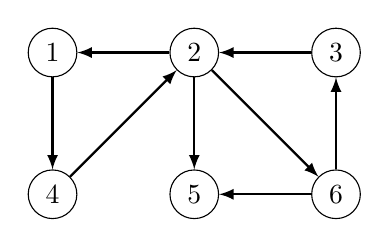
\begin{tikzpicture}[scale=0.9]
\node[draw, circle] (1) at (1,3) {$1$};
\node[draw, circle] (2) at (1,1) {$4$};
\node[draw, circle] (3) at (3,3) {$2$};
\node[draw, circle] (4) at (5,3) {$3$};
\node[draw, circle] (5) at (3,1) {$5$};
\node[draw, circle] (6) at (5,1) {$6$};

\path[draw,thick,->,>=latex] (1) -- (2);
\path[draw,thick,->,>=latex] (2) -- (3);
\path[draw,thick,->,>=latex] (3) -- (1);
\path[draw,thick,->,>=latex] (4) -- (3);
\path[draw,thick,->,>=latex] (3) -- (5);
\path[draw,thick,->,>=latex] (3) -- (6);
\path[draw,thick,->,>=latex] (6) -- (4);
\path[draw,thick,->,>=latex] (6) -- (5);
\end{tikzpicture}
\end{center}
la matriz de adyacencia es
\[
V= \begin{bmatrix}
  0 & 0 & 0 & 1 & 0 & 0 \\
  1 & 0 & 0 & 0 & 1 & 1 \\
  0 & 1 & 0 & 0 & 0 & 0 \\
  0 & 1 & 0 & 0 & 0 & 0 \\
  0 & 0 & 0 & 0 & 0 & 0 \\
  0 & 0 & 1 & 0 & 1 & 0 \\
 \end{bmatrix}.
\]
Ahora, por ejemplo, la matriz
\[
V^4= \begin{bmatrix}
  0 & 0 & 1 & 1 & 1 & 0 \\
  2 & 0 & 0 & 0 & 2 & 2 \\
  0 & 2 & 0 & 0 & 0 & 0 \\
  0 & 2 & 0 & 0 & 0 & 0 \\
  0 & 0 & 0 & 0 & 0 & 0 \\
  0 & 0 & 1 & 1 & 1 & 0 \\
 \end{bmatrix}
\]
contiene el número de caminos de 4 aristas
entre los nodos.
Por ejemplo, $V^4[2,5]=2$,
porque hay dos caminos de 4 aristas
desde el nodo 2 hasta el nodo 5:
$2 \rightarrow 1 \rightarrow 4 \rightarrow 2 \rightarrow 5$
y 
$2 \rightarrow 6 \rightarrow 3 \rightarrow 2 \rightarrow 5$.

\subsubsection{Caminos más cortos}

Usando una idea similar en un gráfico ponderado,
podemos calcular para cada par de nodos el mínimo
longitud de un camino
entre ellos que contiene exactamente $n$ aristas.
Para calcular esto, tenemos que definir la multiplicación de matrices
de una nueva manera, para que no calculemos los números
de caminos, sino que minimicemos las longitudes de los caminos.

\begin{samepage}
Como ejemplo, considera el siguiente gráfico:
\begin{center}
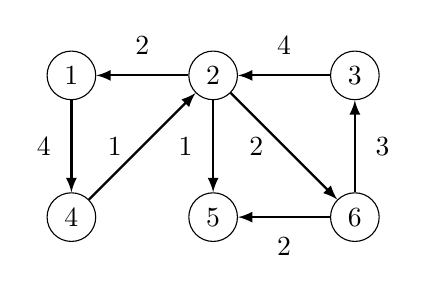
\begin{tikzpicture}[scale=0.9]
\node[draw, circle] (1) at (1,3) {$1$};
\node[draw, circle] (2) at (1,1) {$4$};
\node[draw, circle] (3) at (3,3) {$2$};
\node[draw, circle] (4) at (5,3) {$3$};
\node[draw, circle] (5) at (3,1) {$5$};
\node[draw, circle] (6) at (5,1) {$6$};

\path[draw,thick,->,>=latex] (1) -- node[font=\small,label=left:4] {} (2);
\path[draw,thick,->,>=latex] (2) -- node[font=\small,label=left:1] {} (3);
\path[draw,thick,->,>=latex] (3) -- node[font=\small,label=north:2] {} (1);
\path[draw,thick,->,>=latex] (4) -- node[font=\small,label=north:4] {} (3);
\path[draw,thick,->,>=latex] (3) -- node[font=\small,label=left:1] {} (5);
\path[draw,thick,->,>=latex] (3) -- node[font=\small,label=left:2] {} (6);
\path[draw,thick,->,>=latex] (6) -- node[font=\small,label=right:3] {} (4);
\path[draw,thick,->,>=latex] (6) -- node[font=\small,label=below:2] {} (5);
\end{tikzpicture}
\end{center}
\end{samepage}

Construyamos una matriz de adyacencia donde
$\infty$ significa que una arista no existe,
y otros valores corresponden a pesos de aristas.
La matriz es
\[
V= \begin{bmatrix}
  \infty & \infty & \infty & 4 & \infty & \infty \\
  2 & \infty & \infty & \infty & 1 & 2 \\
  \infty & 4 & \infty & \infty & \infty & \infty \\
  \infty & 1 & \infty & \infty & \infty & \infty \\
  \infty & \infty & \infty & \infty & \infty & \infty \\
  \infty & \infty & 3 & \infty & 2 & \infty \\
 \end{bmatrix}.
\]
En lugar de la fórmula
\[
AB[i,j] = \sum_{k=1}^n A[i,k] \cdot B[k,j]
\]
ahora usamos la fórmula
\[
AB[i,j] = \min_{k=1}^n A[i,k] + B[k,j]
\]
para la multiplicación de matrices, por lo que calculamos
un mínimo en lugar de una suma,
y una suma de elementos en lugar de un producto.
Después de esta modificación,
las potencias de la matriz corresponden a
las rutas más cortas en el gráfico.

Por ejemplo, como
\[
V^4= \begin{bmatrix}
  \infty & \infty & 10 & 11 & 9 & \infty \\
  9 & \infty & \infty & \infty & 8 & 9 \\
  \infty & 11 & \infty & \infty & \infty & \infty \\
  \infty & 8 & \infty & \infty & \infty & \infty \\
  \infty & \infty & \infty & \infty & \infty & \infty \\
  \infty & \infty & 12 & 13 & 11 & \infty \\
 \end{bmatrix},
\]
podemos concluir que la longitud mínima de una ruta
de 4 aristas
desde el nodo 2 hasta el nodo 5 es 8.
Tal ruta es
$2 \rightarrow 1 \rightarrow 4 \rightarrow 2 \rightarrow 5$.

\subsubsection{Teorema de Kirchhoff}

\index{Teorema de Kirchhoff}
\index{árbol de expansión}

\key{Teorema de Kirchhoff}
%\footnote{G. R. Kirchhoff (1824--1887) fue un físico alemán.}
proporciona una forma
de calcular el número de árboles de expansión
de un gráfico como un determinante de una matriz especial.
Por ejemplo, el gráfico
\begin{center}
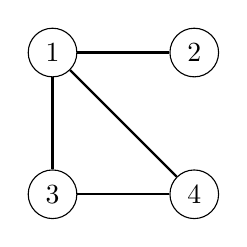
\begin{tikzpicture}[scale=0.9]
\node[draw, circle] (1) at (1,3) {$1$};
\node[draw, circle] (2) at (3,3) {$2$};
\node[draw, circle] (3) at (1,1) {$3$};
\node[draw, circle] (4) at (3,1) {$4$};

\path[draw,thick,-] (1) -- (2);
\path[draw,thick,-] (1) -- (3);
\path[draw,thick,-] (3) -- (4);
\path[draw,thick,-] (1) -- (4);
\end{tikzpicture}
\end{center}
tiene tres árboles de expansión:
\begin{center}
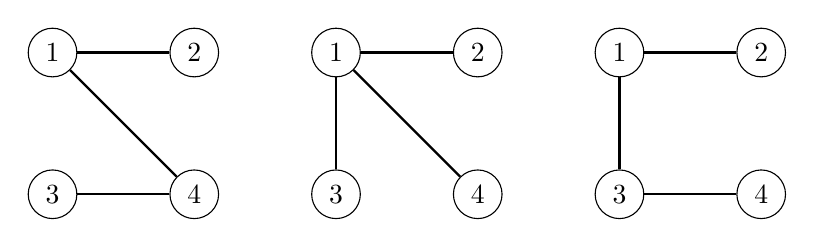
\begin{tikzpicture}[scale=0.9]
\node[draw, circle] (1a) at (1,3) {$1$};
\node[draw, circle] (2a) at (3,3) {$2$};
\node[draw, circle] (3a) at (1,1) {$3$};
\node[draw, circle] (4a) at (3,1) {$4$};

\path[draw,thick,-] (1a) -- (2a);
%\path[draw,thick,-] (1a) -- (3a);
\path[draw,thick,-] (3a) -- (4a);
\path[draw,thick,-] (1a) -- (4a);

\node[draw, circle] (1b) at (1+4,3) {$1$};
\node[draw, circle] (2b) at (3+4,3) {$2$};
\node[draw, circle] (3b) at (1+4,1) {$3$};
\node[draw, circle] (4b) at (3+4,1) {$4$};

\path[draw,thick,-] (1b) -- (2b);
\path[draw,thick,-] (1b) -- (3b);
%\path[draw,thick,-] (3b) -- (4b);
\path[draw,thick,-] (1b) -- (4b);

\node[draw, circle] (1c) at (1+8,3) {$1$};
\node[draw, circle] (2c) at (3+8,3) {$2$};
\node[draw, circle] (3c) at (1+8,1) {$3$};
\node[draw, circle] (4c) at (3+8,1) {$4$};

\path[draw,thick,-] (1c) -- (2c);
\path[draw,thick,-] (1c) -- (3c);
\path[draw,thick,-] (3c) -- (4c);
%\path[draw,thick,-] (1c) -- (4c);
\end{tikzpicture}
\end{center}
\index{matriz laplaciana}
Para calcular el número de árboles de expansión,
construimos una \key{matriz laplaciana} $L$,
donde $L[i,i]$ es el grado del nodo $i$
y $L[i,j]=-1$ si hay una arista entre
los nodos $i$ y $j$, y de lo contrario $L[i,j]=0$.
La matriz laplaciana para el gráfico anterior es la siguiente:
\[
L= \begin{bmatrix}
  3 & -1 & -1 & -1 \\
  -1 & 1 & 0 & 0 \\
  -1 & 0 & 2 & -1 \\
  -1 & 0 & -1 & 2 \\
 \end{bmatrix}
\]

Se puede demostrar que
el número de árboles de expansión es igual
al determinante de una matriz que se obtiene
cuando eliminamos cualquier fila y cualquier columna de $L$.
Por ejemplo, si eliminamos la primera fila
y columna, el resultado es

\[ \det(
\begin{bmatrix}
  1 & 0 & 0 \\
  0 & 2 & -1 \\
  0 & -1 & 2 \\
 \end{bmatrix}
) =3.\]
El determinante siempre es el mismo,
independientemente de qué fila y columna eliminemos de $L$.

Tenga en cuenta que la fórmula de Cayley en el Capítulo 22.5 es
un caso especial del teorema de Kirchhoff,
porque en un gráfico completo de $n$ nodos

\[ \det(
\begin{bmatrix}
  n-1 & -1 & \cdots & -1 \\
  -1 & n-1 & \cdots & -1 \\
  \vdots & \vdots & \ddots & \vdots \\
  -1 & -1 & \cdots & n-1 \\
 \end{bmatrix}
) =n^{n-2}.\]
